\documentclass[a4paper]{article}
\usepackage[UTF8]{ctex}  
\usepackage{geometry}
\usepackage{fontawesome}
\usepackage{titlesec}
\usepackage{enumitem}
\usepackage{xcolor}
\usepackage{hyperref}
\usepackage{graphicx}  % 添加图片支持

% 页面设置
\geometry{left=1.8cm,right=1.8cm,top=1cm,bottom=1cm,includefoot}

% 颜色定义
\definecolor{mainred}{RGB}{204,0,0}
\definecolor{darkgray}{RGB}{73,73,73}

% 超链接设置
\hypersetup{
    colorlinks=true,
    linkcolor=mainred,
    filecolor=mainred,
    urlcolor=darkgray,
}

% 节标题格式
\titleformat{\section}
{\color{mainred}\Large\bfseries}
{}{0em}{\faGraduationCap\quad}[\titlerule]
\titlespacing{\section}{0pt}{10pt}{6pt}

% 设置行距
\linespread{1.15}

\begin{document}
% 移除页码
\pagenumbering{gobble}

% 标题部分
\begin{minipage}{0.75\textwidth}  % 增加左侧宽度
\hspace{-1em}  % 向左缩进
{\huge\bfseries 陈启炜}\medskip

\vspace{0.5em}
\hspace{-0.5em}  % 向左缩进
\begin{tabular}{@{}l@{\hspace{0.5em}}l@{\hspace{4em}}l@{}}
{\color{darkgray}\faPhone} & 131-2312-8852 & {\color{darkgray}\faCalendar} 2003.09.21 \\
{\color{darkgray}\faEnvelope} & qiweic10@sjtu.edu.cn & {\color{darkgray}\faUser} 预备党员 \\
{\color{darkgray}\faGithub} & \href{https://github.com/kiwi142857}{\color{darkgray}kiwi142857} & {\color{darkgray}\faHome} \href{https://kiwi142857.github.io/kiwi142857.githhub.io/}{\color{darkgray}个人主页}
\end{tabular}
\end{minipage}
\begin{minipage}{0.25\textwidth}  % 减小右侧宽度
\hspace{0.5em}  % 向右移动
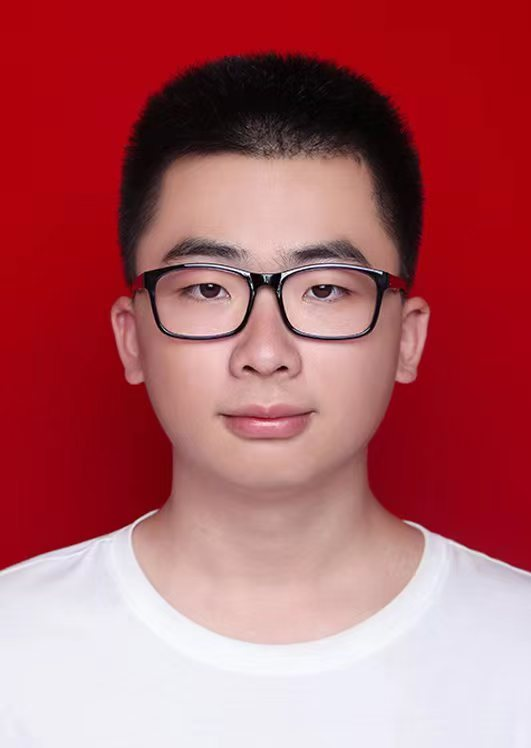
\includegraphics[width=2.8cm]{Kiwi_陈启炜.jpg}
\end{minipage}

\vspace{-2em}
\section*{教育背景}
\noindent\textbf{\large 上海交通大学} \textbf{软件工程专业} \hfill 2022.09 - 至今\\
\vspace{1em}
\textit{学积分: 91.0/100 (专业排名: 7/93)} \hfill \textit{GPA: 3.91/4.30 (专业排名: 12/93)}\\

\vspace{-2em}
\noindent\textbf{主要荣誉}
\begin{itemize}[leftmargin=*,itemsep=0.1em,topsep=-0.1em]
\item 蒋氏奖学金 \hfill 2023-2024学年
\item 上海交通大学优秀本科生奖学金 \hfill 2022-2024学年
\item 上海交通大学优秀团员、优秀学生干部 \hfill 2023-2024学年
\end{itemize}

\section*{项目经历}
\begin{itemize}[leftmargin=*,label={},itemsep=0.5em,topsep=0.2em]
\item \textbf{\href{https://gitee.com/qiweic10/open-trustee_-llm_app}{OpenTrustee LLM}} \hfill \textit{2024.09 - 2024.11}\\
负责基于OpenTrustee和llama.cpp实现大模型在端侧设备的安全推理部署。设计并实现TEE安全环境下的模型加载和推理模块,通过硬件加密保护模型参数安全。针对性能瓶颈。项目获OpenHarmony全国三等奖。

\item \textbf{Tiger 语言编译器} \hfill \textit{2024.09 - 2025.01}\\
独立完成Tiger语言编译器的设计与实现。使用Flex和Bison完成词法分析和语法分析,设计抽象语法树结构实现语义分析。通过栈帧管理和寄存器分配优化实现高效的代码生成。利用LLVM框架实现多级优化,提升生成代码的运行效率。

\item \textbf{\href{https://github.com/kiwi142857/CSE-chfs}{CHFS 分布式文件系统}} \hfill \textit{2024.09 - 2025.01}\\
设计并实现基于GFS架构的分布式文件系统。采用Inode机制管理文件元数据,实现日志机制和快照功能保证数据可靠性。使用Raft算法实现多副本一致性,支持节点故障自动恢复。系统可处理并发请求。

\item \textbf{\href{https://base.sjtu.edu.cn/se/Awards.html}{UniGPT 提示词分享平台}} \hfill \textit{2024.02 - 2024.09}\\
担任{\href{https://github.com/UniGPT-SJTU}{项目}}组长,带领4人团队进行敏捷开发。负责系统架构设计和技术选型,采用微服务架构提升系统可扩展性。实现基于k8s的服务编排和自动化部署流程。通过langchain4j框架集成大模型功能,实现智能提示词推荐。项目获学院软件展示会大二组优胜奖。

\item \textbf{\href{https://github.com/kiwi142857/LSM-Tree}{LSM-Tree KV存储系统}} \hfill \textit{2024.04 - 2024.06}\\
独立完成LSM-Tree KV存储系统的实现。使用C++实现skiplist索引结构,支持高效的插入、删除和查询操作。通过WAL机制保证数据持久化,使用LSM-Tree优化读性能,通过布隆过滤器减少读放大。
\end{itemize}

\section*{校园经历与实习经历}
\hspace{-0.5cm}
\begin{minipage}[t]{0.38\textwidth}
\textbf{学生工作}
\begin{itemize}[leftmargin=*,itemsep=0.1em,topsep=0.1em]
\item 电子信息与电气工程学院学生会成员
\item 班级生活委员
\item 校团委学生组织"思源计划"成员
\end{itemize}
\end{minipage}
\begin{minipage}[t]{0.38\textwidth}
\textbf{社会实践}
\begin{itemize}[leftmargin=*,itemsep=0.1em,topsep=0.1em]
\item "思源潇湘行,图强必知今"社会实践
\item "思源计划"赴粤港澳大湾区社会实践
\end{itemize}
\end{minipage}
\begin{minipage}[t]{0.24\textwidth}
\textbf{实习经历}
\begin{itemize}[leftmargin=*,itemsep=0.1em,topsep=0.1em]
\item 将然科技实习生 \\ 
\textit{2025.01 - 2025.02} \\
\end{itemize}
\end{minipage}

\section*{专业技能}
\begin{itemize}[leftmargin=*,itemsep=0.2em,topsep=0.2em]
\item \textbf{编程语言}:精通C/C++,熟练掌握Python、Java、JavaScript,了解Swift
\item \textbf{开发技能}:微服务架构设计、DevOps、大模型部署优化、安全计算、分布式系统、llama.cpp
\item \textbf{语言能力}:英语六级,技术文档阅读写作能力强
\end{itemize}

\end{document} 